\chapter{Data Structures}


For the sake of completeness a representation of the data structures used in the application will be given.  This will help demonstrate how the objects can be used for both tokens and nodes in the parse tree as well as providing drawing functions and nesting other objects.


\section{Tinctures}



\begin{figure}[H]
  \centering
    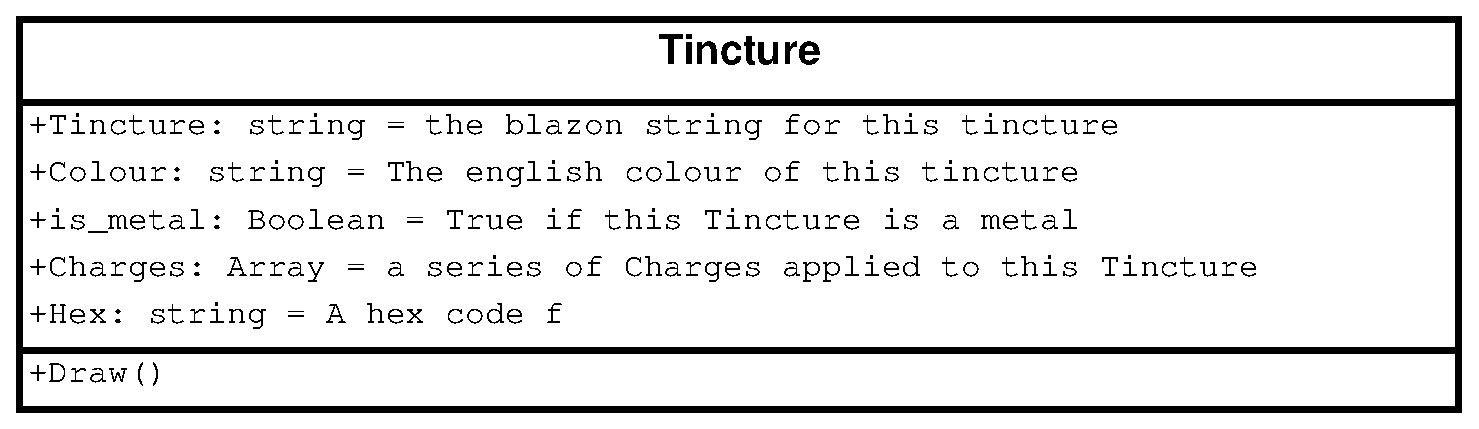
\includegraphics[width=\textwidth]{datastructures/images/tincture.eps}
  \caption{UML description of a Tincture.\cite{linetypes}}
  \label{fig:lines}
  
\end{figure}


\section{Partitions}



\begin{figure}[H]
  \centering
    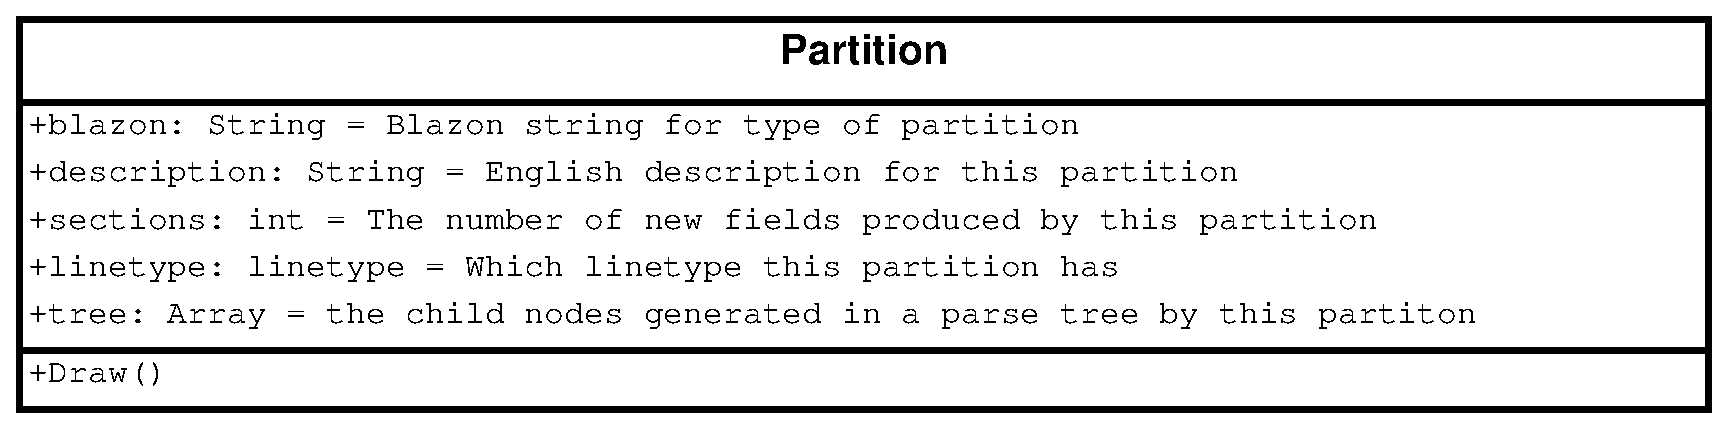
\includegraphics[width=\textwidth]{datastructures/images/partition.eps}
  \caption{UML description of a Partition\cite{linetypes}}
  \label{fig:lines}
  
\end{figure}


\section{Charge}



\begin{figure}[H]
  \centering
    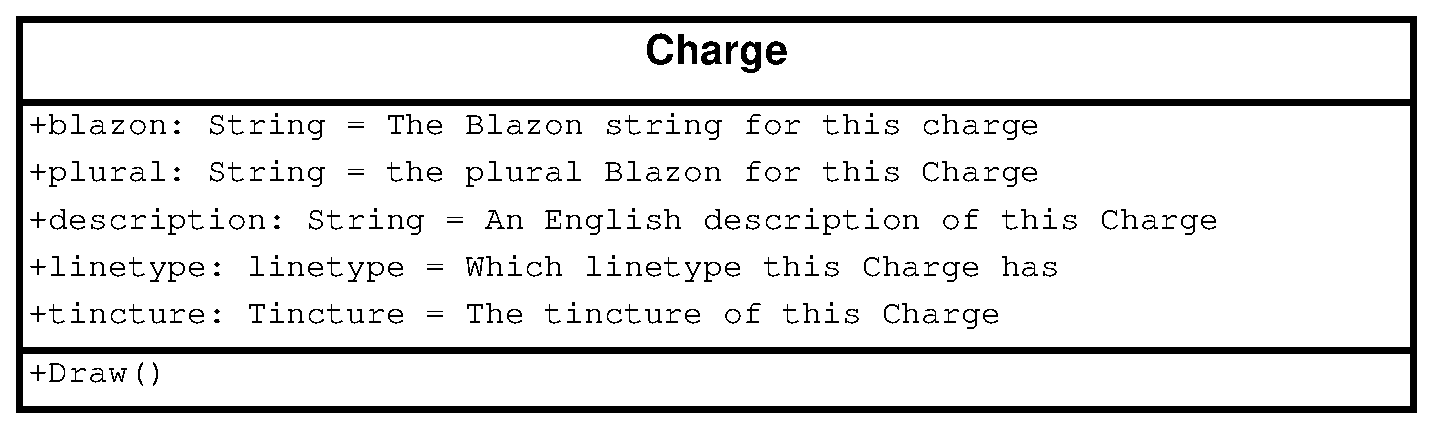
\includegraphics[width=\textwidth]{datastructures/images/charge.eps}
  \caption{UML description of a Charge.\cite{linetypes}}
  \label{fig:lines}
  
\end{figure}

\section{Linetype}



\begin{figure}[H]
  \centering
    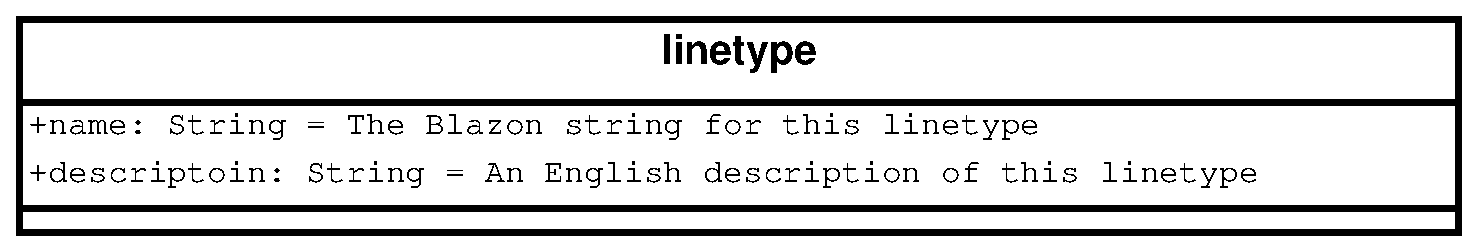
\includegraphics[width=\textwidth]{datastructures/images/linetype.eps}
  \caption{Different line types valid in Blazon.\cite{linetypes}}
  \label{fig:lines}
  
\end{figure}


